\chapter{Vorstellung der vorhandenen Hardware}
\label{sec:Hardware}
Die Hardware besteht im Wesentlichen aus den Komponenten in Abbildung \ref{fig:Übersicht}.
\begin{figure}[htb]
\centering
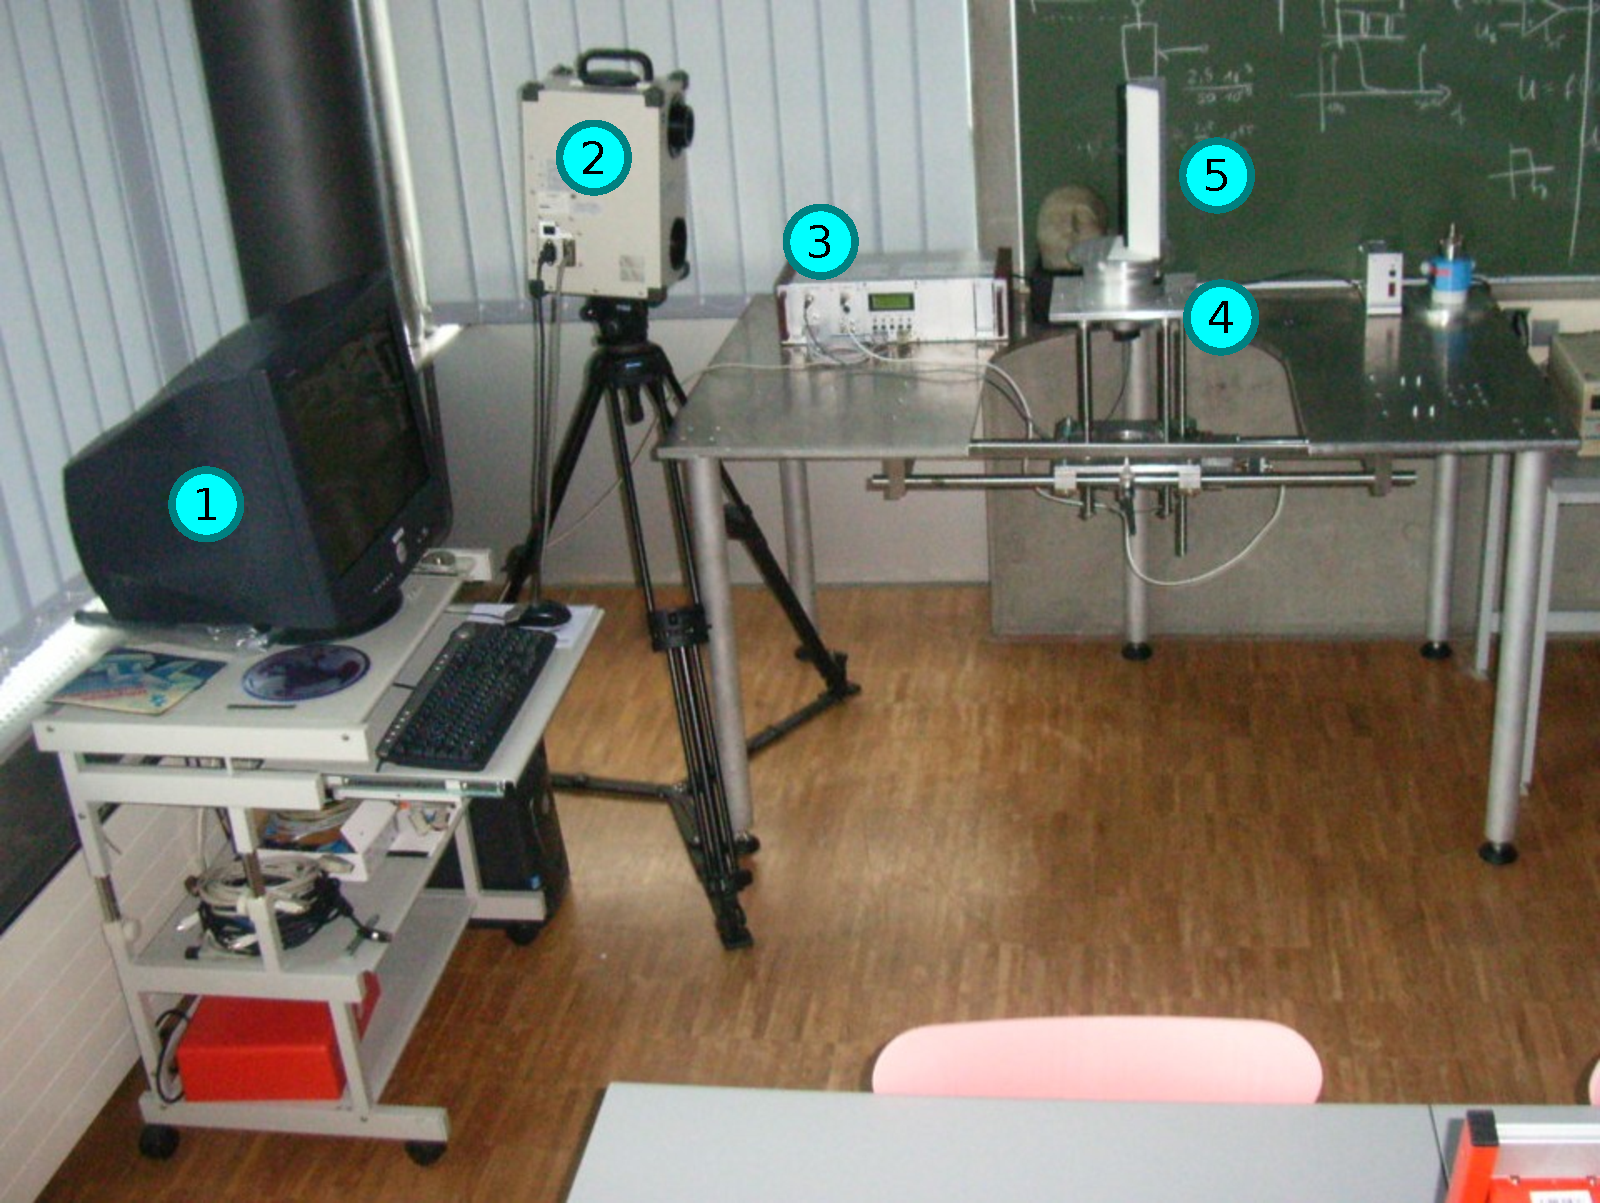
\includegraphics[width=\textwidth]{Uebersicht_2.pdf}
\caption{Blick auf den Arbeitsaufbau}
\label{fig:Übersicht}
\end{figure}
\begin{table}[htb]
\caption{Komponenten im Aufbau}
\begin{tabular}{|c|l|}	\hline 
\rule[-1ex]{0pt}{2.5ex} 1 & 
Computer\\ \hline 
\rule[-1ex]{0pt}{2.5ex} 2 & 
3D-Laserscanner VI-900\\ \hline 
\rule[-1ex]{0pt}{2.5ex} 3 & 
Ansteuerung für den Drehtisch\\ \hline 
\rule[-1ex]{0pt}{2.5ex} 4 & 
Drehtisch\\ \hline 
\rule[-1ex]{0pt}{2.5ex} 5 & 
Zu scannendes Objekt (Kalibrierblech)\\ \hline 
\end{tabular} 
\label{tbl:Aufbau}
\end{table}
\section{Computer}
\label{sec:Computer}
Zur Verfügung steht ein IBM kompatibler x86 Standard PC mit einer \Fachbegriff{SCSI-} und einer \Fachbegriff{RS-232-Schnittstelle}. Auf diesem ist die Erfassungssoftware \emph{RapidForm2004} [\ref{sec:V_Software}] installiert. Die SCSI Schnittstelle wird zur Kommunikation mit dem 3D-Laserscanner und die RS-232-Schnittstelle zur Kommunikation mit einer Schrittmotorsteuerung genutzt.
\section{3D-Laserscanner VI-900}
\label{sec:VI-900}
Der 3D-Laserscanner \emph{VI-900} der Firma \emph{Konica Minolta}[\ref{sec:V_Hardware}] besteht, wie auf Abbildung \ref{fig:VI900} zu sehen, aus einer Kamera und einem \Fachbegriff{Lasertriangulator}. Das System lässt sich über eine SCSI-Schnittstelle ansprechen und konfigurieren. Zur mobilen Nutzung kann das Gerät auch auf der Rückseite bedient werden. Aufgenommene Daten können auf einer \Fachbegriff{CF-Karte} gespeichert werden. Im Projekt wurde jedoch lediglich die direkte Ansteuerung via SCSI genutzt.\\
Der VI-900 digitalisiert Objekte durch ein Laser-Lichtschnittverfahren. Das vom Objekt reflektierte Licht wird von einer CCD-Flächenkamera erfasst, nach Ermittlung der Distanzwerte (Z-Achse) mittels Laser-Triangulation werden die 3D-Daten erstellt. Der Laserstrahl wird mit Hilfe eines hochpräzisen galvanischen Spiegels über das Objekt projiziert, pro Scan werden 640 x 480 Einzelpunkte erfasst.\cite{Minolta:Einleitung}\\
Die Technischen Daten befinden sich im Anhang in Tabelle \ref{tab:TD_VI-910}
\begin{figure}[htb]
\centering
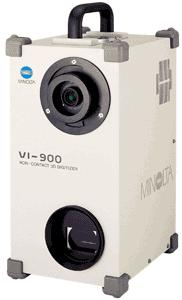
\includegraphics[width=100pt]{vi900-big.jpg}
\caption{VI-900 - Kamera oben, Lasertriangulator unten}
\label{fig:VI900}
\end{figure}
\subsection{Lasertriangulator Prinzip}
\label{sec:LaserTri}
Ein Lasertriangulator besteht, wie in Abbildung \ref{fig:LaserTriangulator} zu sehen, aus einem Laser, einem Linsensystem und im einfachsten Fall, aus einer Pixeldetektorzeile. Der Laser strahlt auf ein Objekt und je nach Entfernung des Objektes wird das Streulicht unter einem anderen Winkel zurückgestrahlt. Das Streulicht wird durch die Linsen auf den Pixeldetektor abgebildet. Über die Position des Laserspots auf dem Pixeldetektor lässt sich auf die Entfernung des Objektes schließen.
\begin{figure}[h]
\centering
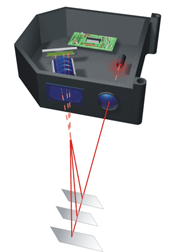
\includegraphics[width=100pt]{Laser-Triangulation.png}
\caption{Prinzip: Laser-Triangulation}
\label{fig:LaserTriangulator}
\end{figure}

\section{Drehtisch und Ansteuerung}
\label{sec:AnsteuerungDrehtisch}
\subsection{Drehtisch}
\label{sec:Drehtisch}
Der Tisch in dem der Drehtisch verbaut ist, ist eine Eigenkonstruktion der Werkstatt des RheinAhrCampus Remagen. Er besteht aus einer massiven Edelstahlarbeitsplatte, welche auf 4 Füßen ruht. Aus dieser ist ein Rechteck mit aufgesetztem Halbkreis ausgeschnitten. In diesem Ausschnitt befindet sich der Drehtisch(siehe Abbildung \ref{fig:Drehtisch}). Er ist auf einem Schienensystem gelagert. Mit dem Schienensystem kann der Drehtisch in der Vertikalen positioniert werden. Mit einem Schrittmotor lässt sich der Drehtisch zusätzlich in der Höhe verstellen. Die Höhenverstellung wird mit einem \Fachbegriff{Schneckengetriebe} realisiert. Ein weiterer Schrittmotor ist für die Drehung des Tisches zuständig. Der Tisch ist über ein \Fachbegriff{Harmonic-Drive-Getriebe} mit dem Schrittmotor verbunden. Das Übersetzungsverhältnis des Getriebes beträgt 1:50.  
\begin{figure}[h]
\centering
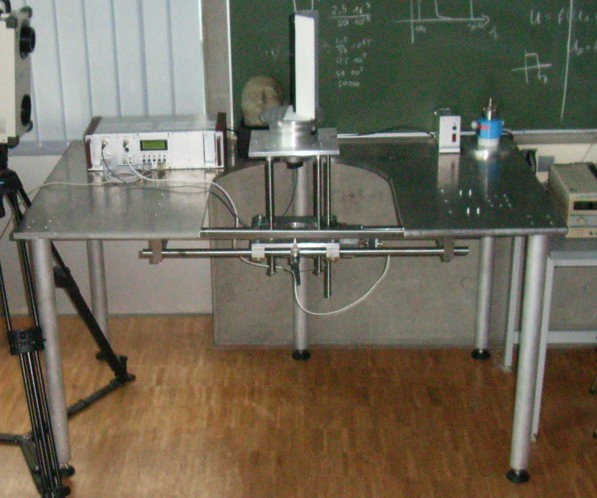
\includegraphics[width=\textwidth]{Drehtisch}
\caption{Drehtisch}
\label{fig:Drehtisch}
\end{figure}
 
\subsection{Spannungsversorgung}
\label{sec:Spannungsv}
Die Schrittmotorkarten werden von einem PC-Netzteil gespeist. Die \Fachbegriff{Logikbausteine} werden mit 5V gespeist, zusätzlich werden die Schrittmotorkarten mit 12V für die Schrittmotoren gespeist. Die Kabel sind direkt an die Verbindungsleisten gelötet.\\
Dies verhindert das einfache Ausbauen der Spannungsversorgung und die einfache Erweiterung um neue Einschubkarten.
\subsection{Schrittmotoren}
\label{sec:Schrittmotoren}
Für die Rotation kommt der Schrittmotor 440-458 der Firma R+S zum Einsatz. Dieser hat einen Schrittwinkel von 1,8°, eine Haltedrehmoment von 500mNm, wird mit 8-Drahtleitung verschaltet und mit 12V Gleichspannung versorgt. Aus dem Schrittwinkel ergeben sich 200 Schritte pro Umdrehung. Diese werden mit einem \Fachbegriff{Harmonic-Drive-Getriebe}, mit einer Übersetzung von 500:1, auf 100.000 Schritte pro Umdrehung erhöht.\\
Für die Höhenverstellung wird der Schrittmotor 440-420, ebenfalls von der Firma R+S, verwendet. Dieser hat auch einen Schrittwinkel von 1,8°, hat jedoch ein Haltemoment von 70mNm, wird in 6-Drahtleitung verschaltet und mit 5V Gleichspannung gespeist. Dieser ist mit einer Übersetzung von 5:1 und einem Schneckengetriebe mit dem Drehtisch verbunden.

\subsection{Schrittmotorkarten}
\label{sec:Schrittmotorkarten}
Die Ansteuerung für die Schrittmotoren sind als 19''-Einschübe realisiert, siehe Abbildung \ref{fig:19Zoll_Rack} links. Für jeden Schrittmotor wird ein Einschub benötigt.
Die Einschübe sind Produkte der Firma R+S. Mittels \Fachbegriff{RS-232 Schnittstelle} lassen sich die Karten konfigurieren und ansteuern. Die Konfiguration und Ansteuerung erfolgt über einen vorgegeben 
\Fachbegriff{ASCII}\footnote{Der American Standard Code for Information Interchange (ASCII, alternativ US-ASCII, oft [æski] ausgesprochen) ist eine 7-Bit-Zeichenkodierung\cite{wiki:ASCII}}
 Befehlssatz. Der Befehlssatz befindet sich im Kapitel \ref{sec:A_ASCII_Befehle}. Es können zwei oder mehr Karten als 
\Fachbegriff{Daisy-Chain}\footnote{Als Daisy Chain (englisch, wörtlich „Gänseblümchenkette“) bezeichnet man eine Anzahl von Hardware-Komponenten, welche in Serie miteinander verbunden sind (meist in sogenannten Bussystemen in der Automatisierungstechnik).\cite{wiki:Daisy} } in Reihe geschaltet werden.\\
Zu Beginn des Projekts war nur die erste Schrittmotorsteuerung vorbereitet.
\begin{figure}[h]
\centering
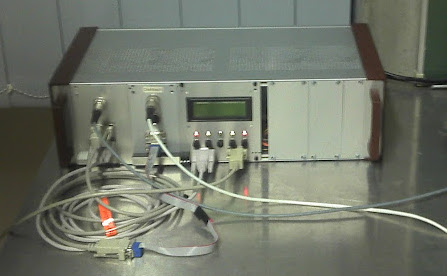
\includegraphics[width=\textwidth]{19Zoll_Rack}
\caption{Ansteuerung im 19''-Rack}
\label{fig:19Zoll_Rack}
\end{figure}
\subsection{Motorverkabelung}
\label{sec:Motorverkabelung}
Die Schrittmotoren benötigen ein mindestens 4-adriges Kabel. Das Kabel für den Schrittmotor, der für die Rotation zuständig ist, war bereits gefertigt. Ein Kabel zwischen Schrittmotor und Schrittmotorkarte zur Höhenverstellung und für die Endschalter war nicht vorhanden und wurde im Verlauf des Projekts gefertigt. 

\subsection{Endschalter}
\label{sec:Endschalter}
Die Schrittmotorkarten unterstützen das Abschalten der Motoren wenn ein sogenannter Endschalter ausgelöst wird. Dies sind im allgemeinen mechanische Schalter die ausgelöst werden wenn der Tisch sich dem Ende des Arbeitsbereiches nähert. Dies verhindert eine Beschädigung des Aufbaus.\\
Im Aufbau sind bereits induktive Endschalter der Firma \textit{Pepperl+Fuchs} verbaut. Diese werden durch einen Metallstutzen ausgelöst. Dieser ist jedoch schlecht positioniert oder ungenügend lang. Würde der Drehtisch über seine Grenzen hinaus in der Höhe verstellt werden, würden die Endschalter nicht rechtzeitig ausgelöst werden und der Aufbau würde beschädigt werden.


\section{Mikrocontroller}
\label{sec:Mikrocontroller}
Ein Mikrocontroller besteht, wie in Abbildung \ref{fig:uC_Blockdiagramm} zu sehen, aus CPU, Flash-Speicher, EEPROM, Registern, Ports und mehreren Peripherie-Funktionen wie z.B. Timern, ADC, DAC und seriellen Schnittstellen. Für unterschiedliche Aufgaben können unterschiedliche Mikrocontroller verwendet werden, welche sich in ihrem Funktionsumfang unterscheiden.\\
Besonders Wichtig im Mikrocontroller sind die sogenannten Register. Dieses sind spezielle, meist 8-Bit breite, Abschnitte im Speicher. Sie repräsentieren Werte und Einstellungen im Mikrocontroller. Diese können  beschrieben und ausgelesen oder nur ausgelesen werden. Durch das Auslesen oder Beschreiben der Register kann der Mikrocontroller mit internen und externen Komponenten interagieren. Die Register die zur externen Kommunikation dienen werden als Ports bezeichnet. \\
Es stand ein ATmega8515 \cite{atmel:8515} im DIL-Gehäuse zur Verfügung. Dieser hatte 8 Kbyte Flash, drei externe Interrupts, eine serielle Schnittstelle und konnte mit bis zu 16 MHz betrieben werden. 
Dieser war geeignet um sich mit den speziellen Eigenheiten der Mikrocontroller Programmierung vertraut zu machen.
\begin{figure}[htb]
\centering
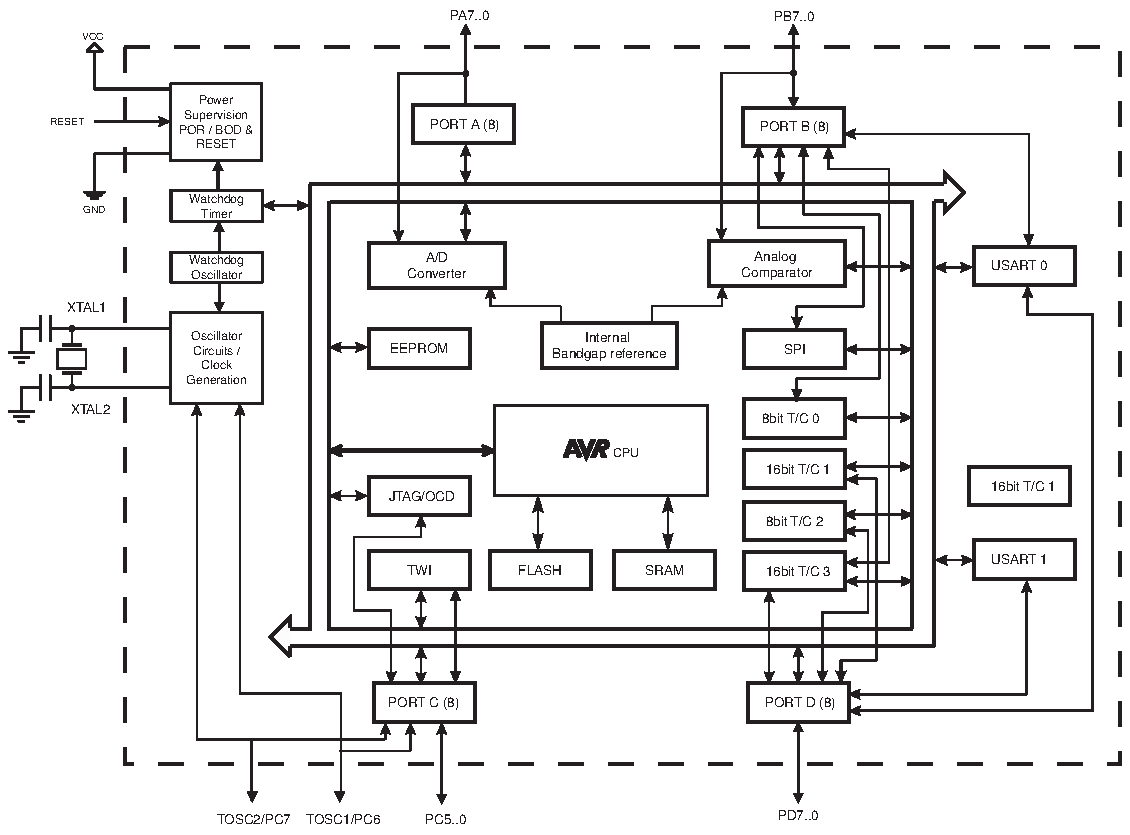
\includegraphics[width=\textwidth]{Mikrocontroller_Block}
\caption{Block Diagramm: Mikrocontroller ATmega324A\cite{atmel:ug_324A}}
\label{fig:uC_Blockdiagramm}
\end{figure}

\subsection{Entwicklerboard STK500}
\label{sec:STK500}
Um den Mikrocontroller zu programmieren und die Programmierung zu überprüfen, wird das \Fachbegriff{Entwicklerboard} \emph{STK500}[\ref{sec:V_Hardware}], wie auf Abbildung \ref{fig:STK500} zu sehen, verwendet. Das Board enthält mehrere Mikrocontroller-Steckplätze, 2 serielle Schnittstellen, 8 Taster, 8 LEDs, 2 Erweiterungsports, eine \Fachbegriff{ISP}\footnote{In System Programmer} Programmierschnittstelle und mehrere Jumper zum Konfigurieren des Boards.\\
Von den beiden seriellen Schnittstellen kann die Eine zur Programmierung des Mikrocontrollers verwendet werden. Die Andere kann zur Kommunikation mit dem Mikrocontroller genutzt werden.\\
Auf dem Board stehen fünf 10 polige Stiftleisten 
zur Verfügung. Diese sind direkt mit den Ein- und Ausgabe Pins, den sogenannten \emph{Ports}, des Mikrocontroller verbunden und können über Flachbandkabel mit Hardwarekomponenten wie z.B. Taster, LED, LC-Displays oder seriellen Schnittstellen verbunden werden.
\begin{figure}[htb]
\centering
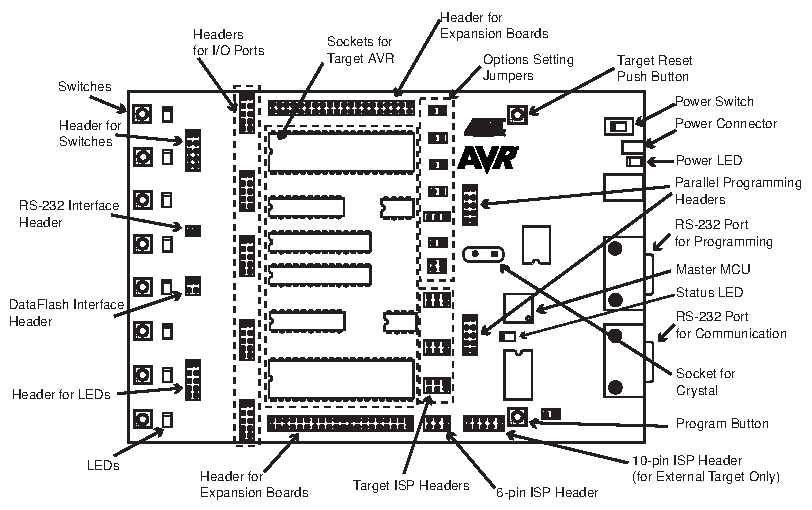
\includegraphics[width=\textwidth]{STK500_Schema.pdf}
\caption{Schemazeichnung eines STK500\cite{atmel:ug_STK500}}
\label{fig:STK500}
\end{figure}

\subsection{AVRISP mkII}
\label{sec:AVRISP}
Der \emph{AVRISP mkII}[\ref{sec:V_Hardware}] ist ein USB-basierter \Fachbegriff{In-System-Programmer}. Dieser kann anstelle des RS-232 basierten Programmiersystem des STK500 verwendet werden.\\
Die Übertragungsgeschwindigkeit des AVRISP mkII ist wesentlich höher als die der seriellen Schnittstelle. 
%Desweiteren wurde der ATmega324A nicht mehr vom STK500 internen ISP unterstützt.\\
Der AVRISP mkII lässt sich einfach an den Programmierport, eine 6-Polige Stiftleiste, des STK500 anschließen.

\subsection{MAX232}
\label{sec:MAX232}
Um die serielle Schnittstelle am Mikrocontroller nutzen zu können, müssen die Spannungspegel auf die des RS-232 Standards gewandelt werden. Dazu befindet sich auf dem STK500 der \Fachbegriff{Pegelwandler} MAX232. 
Dieser wandelt die Spannungspegel des Mikrocontrollers (typ. 0 V -- 5 V \Fachbegriff{TTL}\footnote{Transistor-Transistor-Logik}) auf die Spannungspegel des RS-232 Standards (typ. -12 V -- +12 V).
